\documentclass[dvipdfmx,12pt]{jreport}
\usepackage{tikz, listings}
\usepackage[dvipdfmx]{graphicx}
\usetikzlibrary{shapes,arrows}
\lstset{language={C},%
  basicstyle=\footnotesize,%
  commentstyle=\textit,%
  classoffset=1,%
  keywordstyle=\bfseries,%
  frame=tRBl,framesep=5pt,%
  showstringspaces=false,%
  numbers=left,stepnumber=1,numberstyle=\footnotesize%
}%
\title{ 情報実験第三課題1.A}
\author{情報工学科15\_03602 柿沼 建太郎 \\ 情報工学科 15\_10588 中田 光}
\date{\today}
\begin{document}
\maketitle

\chapter*{各課題担当者}
各課題と担当者を表として以下に示す。
\begin{table}[h]
  \begin{tabular}{|l|c|c|} \hline
    課題番号/名前 & 柿沼 & 中田 \\ \hline \hline
    1 & $\circ$ & $\circ$ \\ \hline
    2 & $\circ$ & $\circ$ \\ \hline
    3 & $\circ$ & $\circ$ \\ \hline
    4 & $\circ$ & $\circ$ \\ \hline
    5(test\_io1) &  & $\circ$ \\ \hline
    5(test\_io2) &  & $\circ$ \\ \hline
    5(test\_calc1) & $\circ$ &  \\ \hline
  \end{tabular}
\end{table}

\chapter*{課題プログラムレポート(1,2,3,4)}

\section*{倍精度乗算}
\subsection*{柿沼}
\subsubsection*{流れについての説明}
使用した変数について,以下に示す。
\begin{table}[h]
  \begin{tabular}{|l|l|l|} \hline
    変数名 & 説明 \\ \hline
    X & 乗算の対象 \\ \hline
    Y & 乗算の対象 \\ \hline
    Z & 乗算の対象(Xの拡張用) \\ \hline
    P & 乗算の結果(下位16bit) \\ \hline
    Q & 乗算の結果(上位16bit) \\ \hline
  \end{tabular}
\end{table}

乗算は筆算式に実現した。
Yを右シフトしながらXを左シフトしていき、Yの末尾が1だった場合にはその時のXの値を結果に加算していく。このとき、Xは16回左にシフトするが、結果は倍精度とするためそのままでは上位16bitの情報が失われてしまう。

そこで、新しくZという変数を使い[Z,X]を32bitの変数として扱うことで倍精度計算を実現した。

以下にフローチャートを示す。
\tikzstyle{if} = [diamond, draw, fill=blue!20,
    text badly centered, inner sep=0pt, aspect=3]
\tikzstyle{block} = [rectangle, draw, fill=blue!20,
text centered, rounded corners, minimum height=3em]
\tikzstyle{line} = [draw, -latex']
\tikzstyle{cloud} = [draw, ellipse,fill=red!20, node distance=3cm, text centered,
    minimum height=2em]
\tikzstyle{cloud2} = [draw, ellipse,fill=green!20, node distance=3cm,
    minimum height=2em]
    
\begin{tikzpicture}[node distance = 3cm, auto]
    % Place nodes
    \node [block](init){Z = P = Q = 0};
    \node [if, below of=init, node distance=3cm] (breakIf) {Y == 0?};
    \node [cloud, right of=breakIf](hlt) {HLT};
    \node [block, below of=breakIf](shiftY){Y $>>=$ 1};
    \node [if, below of=shiftY](eSign){E = 1?};
    \node [block, right of=eSign, node distance=4cm](add){[Q,P] += [Z,X]};
    \node [block, below of=eSign](shiftX){[Z,X]$<<=$1};
    \coordinate [left of=shiftX](leftOfShiftX);
    \coordinate [left of=breakIf](leftOfBreakIf);
    % Draw edges
    \path [line] (init) -- (breakIf);
    \path [line] (breakIf) -- node {yes} (hlt);
    \path [line] (breakIf) -- node {no} (shiftY);
    \path [line] (shiftY) -- (eSign);
    \path [line] (eSign) -- node {yes} (add);
    \path [line] (eSign) -- node {no} (shiftX);
    \path [line, left of=shiftX] (shiftX.west) -- (leftOfShiftX) -- (leftOfBreakIf) -- (breakIf.west);
    \path [line] (add.south) |- (shiftX.east);

\end{tikzpicture}

\subsubsection{工夫点}
[Q,P] += [Z,X]を実現する際、PとXの加算によってあふれたbitがEレジスタに入ることを利用し、加算の後Eレジスタの値が1だった場合には1回INCすることで実現した。

\subsubsection{ソースコードと総命令数}
\lstinputlisting[caption=report1\_1.asm]{./report1_1.asm}
総命令数:26

\subsubsection{異なる入力に対する実行命令ステップ数}
\begin{table}[h]
  \begin{tabular}{|l|l|l|} \hline
    入力($X \times Y$) & ステップ数 \\ \hline
    $11 \times 13$ & 90 \\ \hline
    $0 \times 30$ & 114 \\ \hline
    $30 \times 0$ & 4 \\ \hline
    $65535 \times 65535$ & 403 \\ \hline
  \end{tabular}
\end{table}

\subsubsection{EX3命令セットで改良すべき点}
桁あふれしたときにEレジスタの中身を変えてくれるようなINC命令が欲しいと感じた。
それを別の形で実現しようと考え、1をADDする方法も考えたが、即値が扱えないためそれをするのにも手間がかかる。Eレジスタの中身を変えるINCがなくても、即値を扱える機構さえあれば良いと思う。

\subsection*{中田}
\subsubsection*{流れについての説明}
使用した変数について,以下に示す。
\begin{table}[h]
  \begin{tabular}{|l|l|l|} \hline
    変数名 & 説明 \\ \hline
    X & 乗算の対象 \\ \hline
    W & 乗算の対象(Xの拡張用) \\ \hline
    Y& 乗算の対象 \\ \hline
    P & 乗算の結果(下位16bit) \\ \hline
    Z & 乗算の結果(上位16bit) \\ \hline
  \end{tabular}
\end{table}

乗算は筆算法によって計算している。
また、16bitのXを32bitの[W;X]に拡張することで倍精度計算行っている。
Yを右回転シフトしEレジスタが1の場合は、[Z,P]に[W;X]を加算する。そして、[W;X]を左回転シフトする。
これをYが0になるまで繰り返し、筆算法を実現している。 \\

以下にフローチャートを示す。

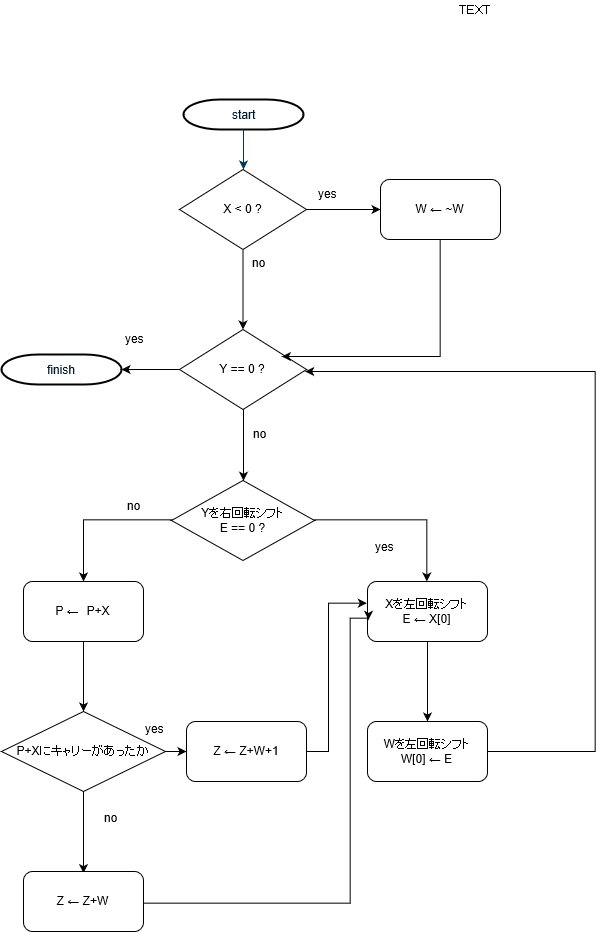
\includegraphics[width=10cm,bb=0 0 604 932]{report1_1_nakata.jpg}


\subsubsection{工夫点}
[P;Z] += [W;X]において、Z += Xの繰り上がりがEレジスタに格納されることを利用して計算した。
Z += Xの計算後、P += Z+Eを計算している。


\subsubsection{ソースコードと総命令数}
\lstinputlisting[caption=report1\_1\_nakata.asm]{./report1_1_nakata.asm}
総命令数:26

\subsubsection{異なる入力に対する実行命令ステップ数}
\begin{table}[h]
  \begin{tabular}{|l|l|l|} \hline
    入力($X \times Y$) & ステップ数 \\ \hline
    $11 \times 13$ & 99 \\ \hline
    $0 \times 30$ & 124 \\ \hline
    $30 \times 0$ & 9 \\ \hline
    $65535 \times 65535$ & 431 \\ \hline
  \end{tabular}
\end{table}

\subsubsection{EX3命令セットで改良すべき点}
桁あふれしたときにEレジスタの中身を変えてくれるようなINC命令が欲しいと感じた。
それを別の形で実現しようと考え、1をADDする方法も考えたが、即値が扱えないためそれをするのにも手間がかかる。Eレジスタの中身を変えるINCがなくても、即値を扱える機構さえあれば良いと思う。

\section*{剰余算}
\subsection*{柿沼}
\subsubsection*{流れについての説明}
使用した変数について,以下に示す。
\begin{table}[h]
  \begin{tabular}{|l|l|l|} \hline
    変数名 & 説明 \\ \hline
    X & 徐算の対象 \\ \hline
    Y & 徐算の対象 \\ \hline
    P & 徐算の商 \\ \hline
    Q & 徐算の余り \\ \hline
    C & 徐算の余り \\ \hline
  \end{tabular}
\end{table}

徐算は筆算式に実現した。
[Q,X]を左シフトしながら商も左シフトしていき、Qに溜まった数がY以上となったときにQからYを引き、商の末尾ビットを立てる。これを16bitぶん繰り返した。 \\

以下にフローチャートを示す。 \\

\begin{tikzpicture}[node distance = 3cm, auto]
    % Place nodes
    \node [block](init){P = Q = 0 \\ C = -16};
    \node [block, below of=init](shift){P $<<=$ 1, [Q,X] $<<=$ 1};
    \node [if, below of=shift] (canSub) {Q $\geq$ Y?};
    \node [block, right of=canSub, node distance=4cm] (sub) {Q -= Y, P++};
    \node [if, below of=canSub, node distance=3cm] (breakIf) {++C == 0?};
    \node [cloud, right of=breakIf](hlt) {HLT};
    \coordinate [left of=breakIf](corner);
    % Draw edges
    \path [line] (init) -- (shift);
    \path [line] (shift) -- (canSub);
    \path [line] (canSub) -- node {yes} (sub);
    \path [line] (canSub) -- node {no} (breakIf);
    \path [line] (sub.south) |- (breakIf.north);
    \path [line] (breakIf) -- node {yes} (hlt);
    \path [line] (breakIf.west) -- node {no} (corner) |- (shift.west);

\end{tikzpicture}

\subsubsection{工夫点}
Q $\geq$ Yの部分でQ-Yを計算するため、それをそのままQ -= Yに転用した。 \\
Q $\geq$ Yの計算は\bf{符号なし16bit}整数として計算しなければならないため、Eレジスタを含めた\bf{符号あり17bit}と考えて、適切な計算の後SZEで判定するという手法をとった。

YをEレジスタを含めた17bit符号あり整数と考えた場合、符号反転後はほとんどの場合最上位ビット(Eレジスタ)が立っていることになるが、唯一Yが0のときのみ符号を反転してもEレジスタは0のままなため、反転前のYに対してSZAでEレジスタの値を定めた。

\subsubsection{ソースコードと総命令数}
\lstinputlisting[caption=report1\_2.asm]{./report1_2.asm}
総命令数:28

\subsubsection{異なる入力に対する実行命令ステップ数}
\begin{table}[h]
  \begin{tabular}{|l|l|l|} \hline
    入力($X \div Y$) & ステップ数 \\ \hline
    $30 \div 7$ & 340 \\ \hline
    $0 \div 15$ & 336 \\ \hline
    $65535 \div 1$ & 400 \\ \hline
    $65535 \div 65535$ & 340 \\ \hline
  \end{tabular}
\end{table}

\subsubsection{EX3命令セットで改良すべき点}
EX3の命令セットでは、スキップ命令が直感に反するものが多いと感じたため、スキップ条件が逆の命令セットがあると書きやすくなると思う。



\subsection*{中田}
\subsubsection*{流れについての説明}
使用した変数について,以下に示す。
\begin{table}[h]
  \begin{tabular}{|l|l|l|} \hline
    変数名 & 説明 \\ \hline
    X & 徐算の対象 計算後、剰余の商を出力 \\ \hline
    Y & 徐算の対象 \\ \hline
    P & 剰余の余り \\ \hline
    W & カウントする変数 \\ \hline
  \end{tabular}
\end{table}

徐算は筆算式によって計算している。
[P;X]を左回転シフトし、PがY以上になったらP-Yをし、Xに商のビットを立てる。
これを16回繰り返す。 \\

以下にフローチャートを示す。 \\

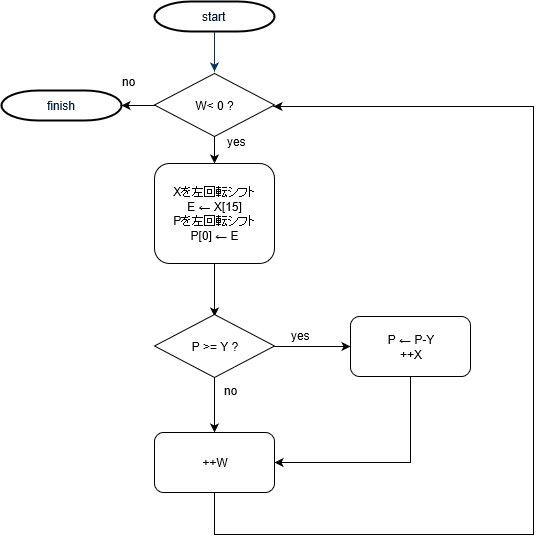
\includegraphics[width=10cm,bb=0 0 542 543]{report1_2_nakata.jpg}



\subsubsection{工夫点}

P$\geq$Yを判定する際にP-Yの正負の判定を用いた。 \\
ここで、P-YをSNAによって判定すると16bit符号あり整数として扱ってしまうため誤りが生じる。 \\
そのため、Eレジスタを17bit目とすることで、16bit符号なし整数として計算を行った。
Eが1の時P-Yを正と判定し、0の時は負と判定する。



\subsubsection{ソースコードと総命令数}
\lstinputlisting[caption=report1\_2\_nakata.asm]{./report1_2_nakata.asm}
総命令数:30

\subsubsection{異なる入力に対する実行命令ステップ数}
\begin{table}[h]
  \begin{tabular}{|l|l|l|} \hline
    入力($X \div Y$) & ステップ数 \\ \hline
    $30 \div 7$ & 362 \\ \hline
    $0 \div 15$ & 336 \\ \hline
    $65535 \div 1$ & 467 \\ \hline
    $65535 \div 65535$ & 362 \\ \hline
  \end{tabular}
\end{table}

\subsubsection{EX3命令セットで改良すべき点}
INC命令によってカウントするためにWを-16としたが、負の数を用いると直感的ではない。 \\
そのため、デクリメントを行う命令が欲しいと感じた。\\

\section*{16進 $\rightarrow$ 10進}
\subsection*{柿沼}
\subsubsection*{流れについての説明}
使用した変数について,以下に示す。
\begin{table}[h]
  \begin{tabular}{|l|l|l|} \hline
    変数名 & 説明 \\ \hline
    OUTPUT & 出力文字列 \\ \hline
    IPT & 入力文字列の先頭へのポインタ \\ \hline
    OPT & 出力文字列の先頭へのポインタ \\ \hline
    EPT & エラー文字列の先頭へのポインタ \\ \hline
    CNT & 文字列のカウント用変数 \\ \hline
    X & 徐算の対象 \\ \hline
    Y & 徐算の対象 \\ \hline
    P & 徐算の商 \\ \hline
    Q & 徐算の余り \\ \hline
    C & 徐算の余り \\ \hline
  \end{tabular}
\end{table}
使用した定数について,以下に示す。
\begin{table}[h]
  \begin{tabular}{|l|l|l|} \hline
    定数名 & 説明 \\ \hline
    TEN & 即値「10」 \\ \hline
    A & 即値「'A'」 \\ \hline
    F & 即値「'F'」 \\ \hline
    ZERO & 即値「'0'」 \\ \hline
    NINE & 即値「'9'」 \\ \hline
    CINIT & 即値「-16」 \\ \hline
    INPUT & 入力文字列 \\ \hline
    ERROR & エラー文字列 \\ \hline
  \end{tabular}
\end{table}

16進数文字列として格納されたINPUTを数値としてXに格納し、1桁ずつOUTPUTに入れていく。
Xへの格納に不備が発生した場合にはERRORをOUTPUTにコピーする。
なお、このプログラムでは出力文字列は逆順に格納される。

以下にフローチャートを示す。 \\

\begin{tikzpicture}[node distance = 2.7cm, auto]
    % Place nodes
    \node [block](init){X=0,CNT = -INPUT.length-1};
    \node [if, below of=init](inputEnd){++CNT == 0?};
    \node [block, below of=inputEnd] (inputInc) {IPT++, X $<<$ 4};
    \node [cloud2, right of=inputEnd, node distance=4.5cm] (output) {to output...};
    \node [if, below of=inputInc] (ifA) {'A' $\leq$ *IPT $\leq$ 'F'};
    \node [if, below of=ifA] (ifN) {'0' $\leq$ *IPT $\leq$ '9'};
    \node [block, left of=ifA, node distance=5.5cm] (la) {X = *IPT - 'A' + 10};
    \node [block, left of=ifN, node distance=5.5cm] (ln) {X = *IPT - '0'};
    \node [block, below of=ifN, text width = 200] (errInit) {*OPT = *EPT, \\ CNT = -ERROR.length-1};
    \node [block, below of=errInit, text width = 100] (errRoot) {OPT++, EPT++, *OPT = *EPT};
    \node [if, below of=errRoot] (errBreak) {++CNT == 0};
    \node [cloud, below of=errBreak, node distance=2cm] (errHlt) {HLT};
    \coordinate [left of=inputInc, left=6cm] (corner);
    \coordinate [left of=errBreak] (corner2);
    % Draw edges
    \path [line] (init) -- (inputEnd);
    \path [line, dashed] (inputEnd) -- node {yes} (output);
    \path [line] (inputEnd) -- node {no} (inputInc);
    \path [line] (inputInc) -- (ifA);
    \path [line] (ifA) -- node{no}(ifN);
    \path [line] (ifN) -- node{no}(errInit);
    \path [line] (errInit) -- (errRoot);
    \path [line] (errRoot) -- (errBreak);
    \path [line] (ifA) -- node {yes}(la);
    \path [line] (ifN) -- node {yes}(ln);
    \path [line] (errBreak) -- node {yes}(errHlt);
    \path [line] (la) -| (corner) -- (inputInc);
    \path [line] (ln) -| (corner) -- (inputInc);
    \path [line] (errBreak) -- node {no}(corner2) |- (errRoot);

\end{tikzpicture}

\begin{tikzpicture}[node distance = 4cm, auto]
    % Place nodes
    \node [block, text width = 120] (outRoot) {OUTPUT.length++ \\ OPT++ \\ P = X / Y \\ Q = X \% Y *OPT = Q};
    \node [if, below of=outRoot] (outBreak) {P == 0 ?};
    \node [block, left of=outBreak] (xp) {X = P};
    \node [cloud, below of=outBreak] (hlt) {HLT};
    \coordinate [above of=outRoot](start);
    \coordinate [left of=outRoot](corner);
    % Draw edges
    \path [line, dashed] (start) -- (outRoot);
    \path [line] (outRoot) -- (outBreak);
    \path [line] (outBreak) -- node {yes} (hlt);
    \path [line] (outBreak) -- node {no} (xp);
    \path [line] (xp) -- (corner) -- (outRoot);

\end{tikzpicture}

\subsubsection{工夫点}
特になし

\subsubsection{ソースコードと総命令数}
\lstinputlisting[caption=report1\_3.asm]{./report1_3.asm}
総命令数:121

\subsubsection{異なる入力に対する実行命令ステップ数}
\begin{table}[h]
  \begin{tabular}{|l|l|l|} \hline
    入力($X$) & ステップ数 \\ \hline
    $0F$ & 783 \\ \hline
    $FFFF$ & 1957 \\ \hline
    $XX$ & 67 \\ \hline
    $ABCX$ & 157 \\ \hline
  \end{tabular}
\end{table}

\subsubsection{EX3命令セットで改良すべき点}
INCの逆で、-1を足す命令が欲しいと感じた。

\subsection*{中田}
\subsubsection*{流れについての説明}
使用した変数について,以下に示す。
\begin{table}[h]
  \begin{tabular}{|l|l|l|} \hline
    変数名 & 説明 \\ \hline
    N & 入力文字列、先頭は文字数 \\ \hline
    PN & 入力文字列へのポインタ \\ \hline
    X & 入力された数を16進数で保持 \\ \hline
    A &  ASCIIコードを16進数に変換した文字列、先頭は文字数 \\ \hline
    PA & Aへのポインタ \\ \hline
    Y & 出力文字列 \\ \hline
    PY & 出力文字列へのポインタ \\ \hline    
    PEMG & エラー文字列へのポインタ \\ \hline
    W & 除算でカウントする変数 \\ \hline
    W1 & Wの初期値を保持 \\ \hline
    COUNT & カウントする変数 \\ \hline
  \end{tabular}
\end{table}
使用した定数について,以下に示す。
\begin{table}[h]
  \begin{tabular}{|l|l|l|} \hline
    定数名 & 説明 \\ \hline
    M & 即値「10」 \\ \hline
    VM1 & 即値「-1」 \\ \hline
    VM48 & 即値「-48」 \\ \hline
    VP48 & 即値「48」 \\ \hline
    VM55 & 即値「-55」 \\ \hline
    VM6 & 即値「-6」 \\ \hline
    VM10 & 即値「-10」 \\ \hline
    EMG & エラー文字列 \\ \hline
    ECNT & エラーの文字数 \\ \hline
  \end{tabular}
\end{table}

ASCIIコードで保持されている文字列Nを16進数文字列Aへと変換し,16進数の数値としてXに保持する。 \\
Xを繰り返し10で割ることで10進数文字列Yへと変換し、それをさらにASCIIコードの文字列へと変換する。 \\
入力された文字列が16進数として扱えない場合はエラーを出力する。 \\
また、入力の16進数には大文字のアルファベットのみを扱うものとし、出力は逆順に出力されるものとする。 \\

以下にフローチャートを示す。 \\

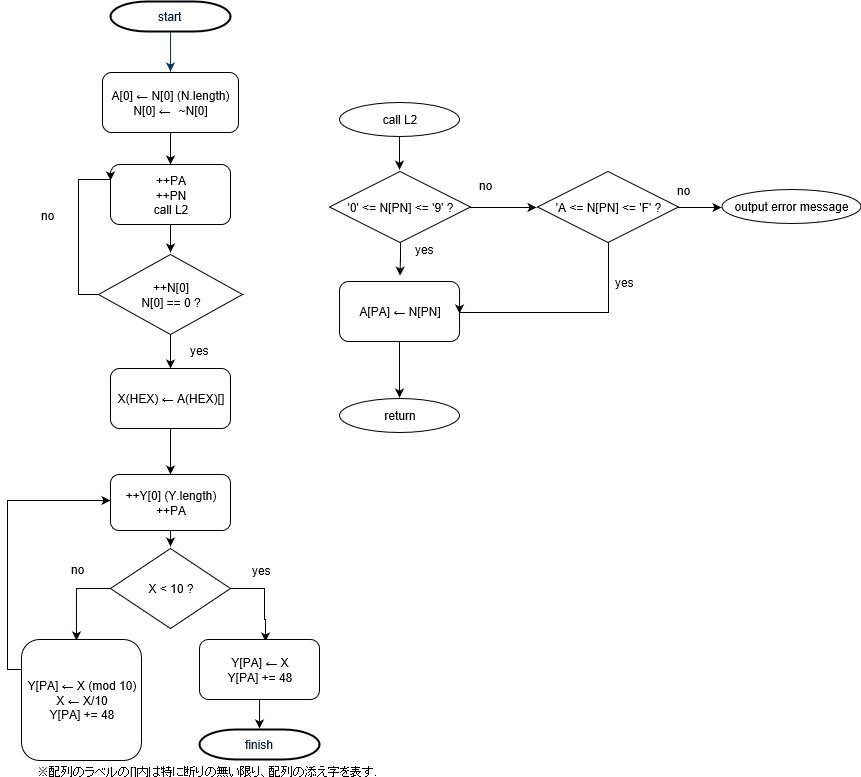
\includegraphics[width=12cm,bb=0 0 861 777]{report1_3_nakata.jpg}}

\subsubsection{工夫点}


\subsubsection{ソースコードと総命令数}
\lstinputlisting[caption=report1\_3\_nakata.asm]{./report1_3_nakata.asm}
総命令数:107

\subsubsection{異なる入力に対する実行命令ステップ数}
\begin{table}[h]
  \begin{tabular}{|l|l|l|} \hline
    入力($X$) & ステップ数 \\ \hline
    $000F$ & 487 \\ \hline
    $FFFF$ & 1724 \\ \hline
    $00XX$ & 74 \\ \hline
    $ABCX$ & 107 \\ \hline
  \end{tabular}
\end{table}

\subsubsection{EX3命令セットで改良すべき点}
即値をADDなどの命令で直接扱えるようにして欲しいと思った。

\section*{素数計算}
\subsection*{柿沼}
\subsubsection*{流れについての説明}
使用した変数について,以下に示す。
\begin{table}[h]
  \begin{tabular}{|l|l|l|} \hline
    変数名 & 説明 \\ \hline
    N & 現在の素数候補 \\ \hline
    M & Nを割る数 \\ \hline
    RES & 結果 \\ \hline
    X & 徐算の対象 \\ \hline
    Y & 徐算の対象 \\ \hline
    P & 徐算の商 \\ \hline
    Q & 徐算の余り \\ \hline
    C & 徐算の余り \\ \hline
  \end{tabular}
\end{table}
使用した定数について,以下に示す。
\begin{table}[h]
  \begin{tabular}{|l|l|l|} \hline
    定数名 & 説明 \\ \hline
    CINIT & 即値「-16」 \\ \hline
  \end{tabular}
\end{table}

自然数Nが素数であるかの判定にはN未満の自然数すべてに対して徐算を実行することで実現した。

以下にフローチャートを示す。 \\

\begin{tikzpicture}[node distance = 2cm, auto]
    % Place nodes
    \node [block](init){RES = 0};
    \node [if, below of=init](assert){N $\leq$ 1};
    \node [cloud, right of=assert] (hltAssert) {HLT};
    \node [block, below of=assert](setM){M = N - 1};
    \node [if, below of=setM] (isPrime) {M == 1?};
    \node [block, right of=isPrime, node distance = 4cm] (res) {RES = N};
    \node [cloud, right of=res] (hlt) {HLT};
    \node [block, below of=isPrime, text width = 100] (div) {P = N / M, \\ Q = N \% M};
    \node [if, below of=div] (isNotPrime) {Q == 0?};
    \node [block, left of=div, node distance = 4cm] (decM) {M = M - 1};
    \node [block, below of=isNotPrime] (decN) {N = N - 1};
    \coordinate [left of=decN, node distance = 6cm](corner);
    % Draw edges
    \path [line] (init) -- (assert);
    \path [line] (assert) -- node {yes}(hltAssert);
    \path [line] (assert) -- node {no} (setM);
    \path [line] (setM) -- (isPrime);
    \path [line] (isPrime) -- node {yes} (res);
    \path [line] (isPrime) -- node {no} (div);
    \path [line] (res) -- (hlt);
    \path [line] (div) -- (isNotPrime);
    \path [line] (isNotPrime) -- node {yes}(decN);
    \path [line] (isNotPrime.west) -| node {no}(decM.south);
    \path [line] (decM.north) |- (isPrime.west);
    \path [line] (decN.west) -- (corner) |- (setM.west);

\end{tikzpicture}

\subsubsection{工夫点}
Q $\geq$ Yの部分でQ-Yを計算するため、それをそのままQ -= Yに転用した。 \\
Q $\geq$ Yの計算は\bf{符号なし16bit}整数として計算しなければならないため、Eレジスタを含めた\bf{符号あり17bit}と考えて、適切な計算の後SZEで判定するという手法をとった。

YをEレジスタを含めた17bit符号あり整数と考えた場合、符号反転後はほとんどの場合最上位ビット(Eレジスタ)が立っていることになるが、唯一Yが0のときのみ符号を反転してもEレジスタは0のままなため、反転前のYに対してSZAでEレジスタの値を定めた。

\subsubsection{ソースコードと総命令数}
\lstinputlisting[caption=report1\_4.asm]{./report1_4.asm}
総命令数:72

\subsubsection{異なる入力に対する実行命令ステップ数}
\begin{table}[h]
  \begin{tabular}{|l|l|l|} \hline
    入力($N$) & ステップ数 \\ \hline
    $2$ & 27 \\ \hline
    $64$ & 61307 \\ \hline
    $255$ & 337101 \\ \hline
    $65535$ & 245377052 \\ \hline
  \end{tabular}
\end{table}

\subsubsection{EX3命令セットで改良すべき点}
可変長のデータを保持する機能がないので、何か方法が欲しいと思った。
スタックなどがあればよいが、簡単さを重視した命令セットでは難しいのかもしれない。

\subsection*{中田}
\subsubsection*{流れについての説明}
使用した変数について,以下に示す。
\begin{table}[h]
  \begin{tabular}{|l|l|l|} \hline
    変数名 & 説明 \\ \hline
    N & 入力および素数の候補、処理終了後において結果 \\ \hline
    N1 & Nを計算の間、保持する \\ \hline
    Y & 最初に割る数(2) \\ \hline
    Y1 & 割る数 \\ \hline
    R & 徐算の余り \\ \hline
    W & 徐算でカウントする変数 \\ \hline
    W & W1の初期値を保持 \\ \hline
  \end{tabular}
\end{table}
使用した定数について,以下に示す。
\begin{table}[h]
  \begin{tabular}{|l|l|l|} \hline
    定数名 & 説明 \\ \hline
    VM1 & 即値「-1」 \\ \hline
  \end{tabular}
\end{table}

自然数Nが素数であるかの判定にはN未満の自然数すべてに対して徐算を実行することで実現した。

以下にフローチャートを示す。 \\

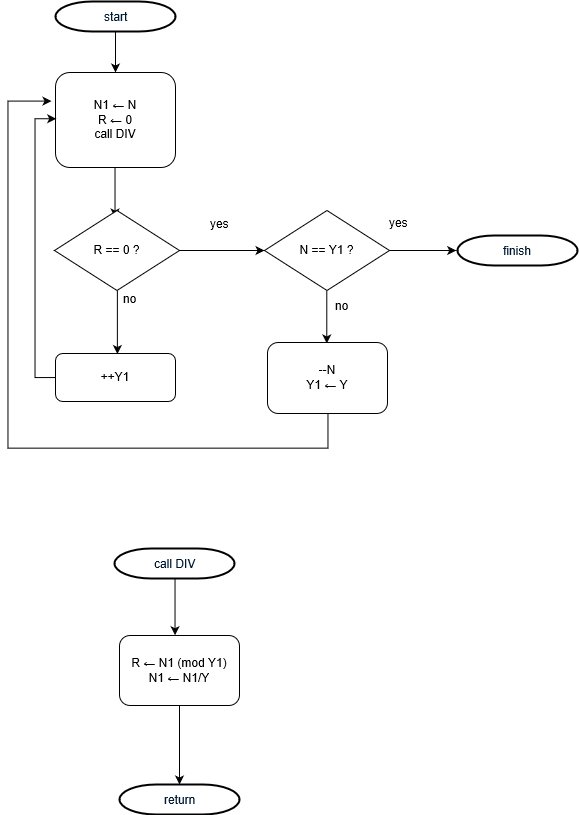
\includegraphics[width=10cm,bb=0 0 579 815]{report1_4_nakata.jpg}}

\subsubsection{工夫点}
Q $\geq$ Yの部分でQ-Yを計算するため、それをそのままQ -= Yに転用した。 \\
Q $\geq$ Yの計算は\bf{符号なし16bit}整数として計算しなければならないため、Eレジスタを含めた\bf{符号あり17bit}と考えて、適切な計算の後SZEで判定するという手法をとった。

YをEレジスタを含めた17bit符号あり整数と考えた場合、符号反転後はほとんどの場合最上位ビット(Eレジスタ)が立っていることになるが、唯一Yが0のときのみ符号を反転してもEレジスタは0のままなため、反転前のYに対してSZAでEレジスタの値を定めた。

\subsubsection{ソースコードと総命令数}
\lstinputlisting[caption=report1\_4\_nakata.asm]{./report1_4_nakata.asm}
総命令数:57

\subsubsection{異なる入力に対する実行命令ステップ数}
\begin{table}[h]
  \begin{tabular}{|l|l|l|} \hline
    入力($N$) & ステップ数 \\ \hline
    $2$ & 378 \\ \hline
    $64$ & 24240 \\ \hline
    $255$ & 100047 \\ \hline
    $65535$ & 24769799 \\ \hline
  \end{tabular}
\end{table}

\subsubsection{EX3命令セットで改良すべき点}



\chapter*{サンプルプログラム解析レポート(5)}
\section{test\_calc1.asm}
\subsection{プログラムの概要}
入力された数値の計算をさせるプログラムである。
ユーザーは最大4桁の16進数表記の数値の足し算と引き算ができる。オーバーフローやアンダーフローは無視し、下位16bitを答えとして出力する。
入力する数値が4桁を超えたりするとエラー文を出力して終了する。

\subsubsection{各サブルーチンの機能}

\begin{table}[h]
  \begin{tabular}{|l|p{10cm}|} \hline
    サブルーチン名 & 機能の説明 \\ \hline
    INI & プログラム本体のエントリーポイント。各種変数の初期化をした後、入力可能状態で待機し、BYEが1になると停止する。 \\ \hline
    INI\_ST & 各種変数の初期化 \\ \hline
    ST0 & 割り込みハンドラのエントリーポイント \\ \hline
    CHK\_CH & ACとTMIが等しいかどうかを返す。 \\ \hline
    SET\_MSG & PTR\_MGにACの指すアドレスを入れ、その指す文字列長をCNTに入れる。 \\ \hline
    READ\_HX & TMIに入った文字が16進数として有効な文字ならHXIにその値を入れ、AC $\geq$にする。無効ならAC$<$0にする。このとき、文字が改行文字ならば=に置き換える。 \\ \hline
    CHK\_DGT & 引数としてACとその他に2つの定数をとり、ACがそれらの間に入っているかどうかを返す。 \\ \hline
    WRITE\_Z & Zに入った数値を文字列としてZMGに入れる。\\ \hline
  \end{tabular}
\end{table}

\subsubsection{処理の流れ}
\scalebox{0.8}[0.8]{
\begin{tikzpicture}[node distance = 2.5cm, auto]
    \coordinate [](entry);
    \node [block, below of=entry, text width=150](init){各種変数初期化 \\ IMSK = 1000 \\ IOT = 1};
    \node [if, below of=init](breakIf){BYE=0?};
    \node [cloud, right of=breakIf](hlt){HLT};
    % Draw edges
    \path [line, dashed] (entry) -- (init);
    \path [line] (init) -- (breakIf);
    \path [line] (breakIf.south) -- node{yes} +(0,-1) -- +(-2,-1) |- (breakIf.west);
    \path [line] (breakIf.east) -- node{no} (hlt);
    \end {tikzpicture}
  }

\scalebox{0.6}[0.6]{
\begin{tikzpicture}[node distance = 2.5cm, auto]
    % Place nodes
    \coordinate [below of=breakIf](entry2);
    \node [block, below of=entry2](start){AC,Eを退避};
    \node [if, below of=start](isOutStt){OUT\_STT $\geq$ 1?};
    \node [if, below of=isOutStt](canInput){FGI == 0?};
    \node [block, below of=canInput](input){入力を取得};
    \node [if, below of=input](isNumber){入力が16進数か?};
    \node [if, below of=isNumber](isOver){STT == 0?};
    \node [block, below of=isOver, text width=200](inputY){Yに入力された数値を追加 \\ Y\_PD = 1};
    \node [cloud2, right of=isOutStt, node distance=4cm](toOut){出力};
    \node [cloud2, right of=isNumber, node distance=4cm](toOpr){計算};
    \node [cloud, left of=canInput, node distance=7cm](irt1){AC,Eを戻す};
    \node [cloud, left of=inputY, node distance=7cm](irt2){AC,Eを戻す};
    \node [cloud, left of=isOver, node distance=7cm, text width=150](err1){PTR\_MG = A\_EMG \\ OUT\_STT = 1 \\ IMSK = 0100};
    % Draw edges
    \path [line, dashed] (entry2) -- (start);
    \path [line] (start) -- (isOutStt);
    \path [line] (isOutStt) -- node {yes} (toOut);
    \path [line] (isOutStt) -- node {no} (canInput);
    \path [line] (canInput) -- node {yes} (irt1);
    \path [line] (canInput) -- node {no} (input);
    \path [line] (input) -- (isNumber);
    \path [line] (isNumber) -- node {yes} (isOver);
    \path [line] (isNumber) -- node {no} (toOpr);
    \path [line] (isOver) -- node {yes} (inputY);
    \path [line] (isOver) -- node {no} (err1);
    \path [line] (inputY) -- (irt2);
\end{tikzpicture}
}

\newpage

\scalebox{0.8}[0.8]{
\begin{tikzpicture}[node distance = 2.5cm, auto]
    % Place nodes
    \node [cloud2](entryOut){出力};
    \node [if, below of=entryOut](canOutput){FGO == 0?};
    \node [if, below of=canOutput](isOut1){OUT\_STT == 1?};
    \node [if, below of=isOut1](isOut2){OUT\_STT == 2?};
    \node [block, below of=isOut2, text width=150](out3){改行文字を出力 \\変数初期化 \\BYE = NXT\_BYE};
    \node [if, below of=out3](isBye){BYE == 1 ?};
    \node [block, below left of=isBye](enableInput){IMSK = 1000};
    \node [block, below right of=isBye](disable){IMSK = 0000};
    \node [cloud, below right of=enableInput](irt1){AC,Eを戻す};
    \node [cloud, left of=canOutput, node distance=4cm](irt2){AC,Eを戻す};
    \node [block, right of=isOut1, text width=100, node distance=5cm](out1){改行文字を出力 \\ OUT\_STT++};
    \node [cloud, right of=out1, node distance=5cm](irt3){AC,Eを戻す};
    \node [block, right of=isOut2, text width=150, node distance=6.5cm](out2){PTR\_MGを全て出力 \\ OUT\_STT++};
    \node [cloud, right of=out2, node distance=5cm](irt4){AC,Eを戻す};
    % Draw edges
    \path [line] (entryOut) -- (canOutput);
    \path [line] (canOutput) -- node {yes}(isOut1);
    \path [line] (canOutput) -- node {no}(irt2);
    \path [line] (isOut1) -- node {yes}(out1);
    \path [line] (isOut1) -- node {no}(isOut2);
    \path [line] (isOut2) -- node {yes}(out2);
    \path [line] (isOut2) -- node {no}(out3);
    \path [line] (out3) -- (isBye);
    \path [line] (isBye) -- node {yes}(enableInput);
    \path [line] (isBye) -- node {no}(disable);
    \path [line] (enableInput) -- (irt1);
    \path [line] (disable) -- (irt1);
    \path [line] (out1) -- (irt3);
    \path [line] (out2) -- (irt4);
\end{tikzpicture}
}

\newpage
\scalebox{0.6}[0.6]{
\begin{tikzpicture}[node distance = 2.5cm, auto]
    % Place nodes
    \node [cloud2](entryOpr){計算};
    \node [if, below of=entryOpr](isWS){入力文字は空白か?};
    \node [if, below of=isWS, node distance=5cm](isOp){入力文字は「+」「-」「=」のいずれかか?};
    \node [block, below of=isOp](swap){入力記号を保存};
    \node [if, below of=swap](isPd){Y\_PD == 0?};
    \node [block, below right of=isPd](setY){Y = X};
    \node [if, below of=isPd, node distance=5cm](switchOp){1つ前の入力記号はどれか?};
    \node [block, below left of=switchOp, node distance=5cm](eq){Z = Y};
    \node [block, below of=switchOp, node distance=5cm](add){Z = X + Y};
    \node [block, below right of=switchOp, node distance=5cm](sub){Z = X - Y};
    \node [block, below of=add, text width=150](beforeWriteZ){X = Z \\ Y = Y\_PD = 0};
    \node [if, below of=beforeWriteZ](isSkipOut){1つ前の記号の記号は「=」か?};
    \node [cloud, below left of=isSkipOut, node distance=5cm, text width=150](writeZ){ZMGにZを書き込む \\ PTR\_MG = A\_ZMG \\ OUT\_STT = 1 \\ IMSK = 0100};
    \node [cloud, below right of=isSkipOut, node distance=5cm](skipout){各種変数を初期化};
    \node [if, right of=isWS, node distance=5cm](isPd2){Y\_PD == 0?};
    \node [if, below right of=isPd2](ws){STT = 1};
    \node [cloud, right of=isPd2, node distance=7cm](irt){復帰};
    \node [cloud, right of=isOp, node distance=10cm, text width=150](err){PTR\_MG = A\_BMG \\ OUT\_STT = 1 \\\ IMSK = 0100};
    % Draw edges
    \path [line] (entryOpr) -- (isWS);
    \path [line] (isWS) -- node{yes}(isPd2);
    \path [line] (isWS) -- node{no}(isOp);
    \path [line] (isPd2) -- node {yes}(irt);
    \path [line] (isPd2) -- node {no}(ws);
    \path [line] (ws) -- (irt);
    \path [line] (isOp) -- node {yes}(swap);
    \path [line] (isOp) -- node {no}(err);
    \path [line] (swap) -- (isPd);
    \path [line] (isPd) -- node {yes}(setY);
    \path [line] (isPd) -- node {no}(switchOp);
    \path [line] (setY) -- (switchOp);
    \path [line] (switchOp) -- node {=}(eq);
    \path [line] (switchOp) -- node {+}(add);
    \path [line] (switchOp) -- node {-}(sub);
    \path [line] (eq) -- (beforeWriteZ);
    \path [line] (add) -- (beforeWriteZ);
    \path [line] (sub) -- (beforeWriteZ);
    \path [line] (beforeWriteZ) -- (isSkipOut);
    \path [line] (isSkipOut) -- node {yes}(skipout);
    \path [line] (isSkipOut) -- node {no}(writeZ);
\end{tikzpicture}
}

\end{document}
